% E.12 矩形 AB=6, AD=8. 沿 EF 折，A 落到 BC 上 A'. E 在 AB, F 在 AD.
% A(0,0), B(6,0), C(6,8), D(0,8). 示例: A' 为 BC 中点 → A'=(6,4), BA'=4.
% BE² + BA'² 关系? 折叠: AE=A'E. 在 △BEA': BE²+4²=AE²=(6-BE)² → BE = 1.25 → E=(1.25,0)
% AF=A'F. 设 AF=t, F=(0,t). A'F²=(6-0)²+(4-t)²=36+(4-t)². AF²=t².
% t²=36+(4-t)² → t²=36+16-8t+t² → 8t=52 → t=6.5 → F=(0,6.5)
\documentclass[tikz,border=4pt]{standalone}
\usepackage{ctex}
\usepackage{amsmath}
\usetikzlibrary{calc}
\begin{document}
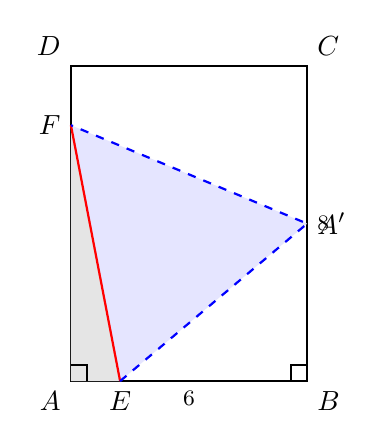
\begin{tikzpicture}[scale=0.5, thick]
  \coordinate (A) at (0,0);
  \coordinate (B) at (6,0);
  \coordinate (C) at (6,8);
  \coordinate (D) at (0,8);
  \coordinate (E) at (1.25,0);
  \coordinate (F) at (0,6.5);
  \coordinate (Ap) at (6,4);

  \draw (A)--(B)--(C)--(D)--cycle;
  % 原 △AEF (灰)
  \fill[black!10] (A)--(E)--(F)--cycle;
  % 折后 △A'EF (蓝虚)
  \fill[blue!10] (Ap)--(E)--(F)--cycle;
  \draw[red, thick] (E)--(F);
  \draw[blue, dashed, thick] (E)--(Ap)--(F);

  % 直角 ∠A
  \draw ($(A)+(0.4,0)$)--($(A)+(0.4,0.4)$)--($(A)+(0,0.4)$);
  % ∠B
  \draw ($(B)+(-0.4,0)$)--($(B)+(-0.4,0.4)$)--($(B)+(0,0.4)$);

  \node[below left] at (A) {$A$};
  \node[below right] at (B) {$B$};
  \node[above right] at (C) {$C$};
  \node[above left] at (D) {$D$};
  \node[below] at (E) {$E$};
  \node[left] at (F) {$F$};
  \node[right] at (Ap) {$A'$};

  \node[below, font=\footnotesize] at ($(A)!0.5!(B)$) {$6$};
  \node[right, font=\footnotesize] at ($(B)!0.5!(C)$) {$8$};
\end{tikzpicture}
\end{document}
